\documentclass[12pt, a4paper]{article}
\usepackage[utf8]{inputenc}
\usepackage[czech]{babel}
\usepackage[left=2.5cm,text={16cm, 24cm},top=3cm]{geometry}
\usepackage{amsmath}
\usepackage{graphicx}
\usepackage{float}
\usepackage{pgfplots}

\begin{document}
\begin{center}
	\begin{huge}\textbf{Výpočet úrovně vrcholu}\end{huge} \\
	\vspace{0.4cm}
	Tomáš Blažek (xblaze31) \\
	\textit{PRL - Paralelní a Distribuované algoritmy} \\
	\textit{Fakulta Informačních Technologií, Brno} \\
\end{center}
 

\section{Rozbor a analýza algoritmu}
\label{sec:rozbor}
Algoritmus pro Výpočet úrovně vrcholu je algoritmus, který pracuje s binárním stromem, který má místo jedné orientované hrany mezi dvěma uzly hned dvě orientované hrany, a to jednu dopřednou a druhou zpětnou, přičemž procesory reprezentují hrany vedoucí grafem. Počet použitých procesorů je závislý od počtu uzlů grafu $n$. Celkový počet procesorů je tedy roven $p = 2n-2$, což udává prostorovou složitost $O(n)$. Každému procesoru přiřadíme index a první polovina indexů procesorů bude znázorňovat dopředné hrany a druhá polovina hrany zpětné. Algoritmus pracuje tak, že nejprve si každá hrana zjistí svoji váhu (1 nebo -1), zdali je dopředná (-1) nebo zpětná (1), a to dokážeme určit v konstantním čase, tedy dostaneme časovou složitost $O(c)$. Dále podle algoritmu vypočteme váhu jednotlivých hran za pomoci paralelního algoritmu Suffix Sum, který bude pracovat s polem následníků tvořeného podle Eulerovy cesty. Za použití Eulerovy cesty vznikne takový graf, který obsahuje orientovanou kružnici, která prochází každou hranou právě jednou.

Následníka Eulerovy cesty lze určit na základě pravidel dvou úrovní. V první úrovni se zjišťuje, zdali je hrana dopředná nebo zpětná  $O(c)$. Pokud je hrana dopředná, tak se zjišťuje, zdali uzel na nějž hrana míří, má levé syna. V případě, že levého syna má, tak následník $next(x)$ má index $next(x)=x+(n-1)$. V opačném případě má následník index $next(x)=2\cdot(x+1)$. Ovšem pokud je hrana zpětná, tak se zjišťuje, zdali uzel na nějž zpětná hrana míří, má pravého syna. Pokud má uzel pravého syna a hrana nevychází z daného pravého syna, tak index následníka je roven $next(x)=x-(n-1)+1$. V opačném případě je následníkův index $next(x)=((x-n-1)/2)-1$, až na výjimku, kde pokud hrana míří na kořenový uzel, tak její následník je daná hrana (kvůli algoritmu Suffix Sum). Z toho plyne, že výpočet následníka podle Eulerovy cesty má konstantní časovou náročnost $O(c)$.

Paralelní algoritmus Suffix Sum má tedy připravené inicializační pole následníků a připraví se tedy ještě pole hodnot, kde hodnota na indexu je rovna váze hrany, kromě hrany jejíž následník je hrana samotná. Ta má potom hodnotu 0. Tedy časová náročnost tohoto kroku je konstantní $O(c)$. Další krok je samotný výpočet sumy suffixů a ten pracuje v $log_{2}(n)$ krocích, jelikož v každém dalším kroku je možné využít výsledků následníka. Jelikož posuv je vždy na následníka následníka, tak se krok vždy zdvojnásobuje s každou iterací, proto stačí použít pouze $log_{2}(n)$ kroků, tedy časová náročnost je $O(log_{2}(n))$. Poslední krok algoritmu Suffix Sum je korekční, kdy se přičte všem členům hodnota poslední hrany Eulerovy cesty, která byla na začátku nahrazena hodnotou 0, což má konstantní časovou náročnost $O(c)$. Celkově tedy algoritmus Suffix Sum má časovou náročnost $t(n)=O(c)*O(log_{2}(n))*O(c)=O(log_{2}(n))$.

Poslední krok algoritmu pro výpočet úrovně vrcholu je korekce výsledku, která přičte ke všem hodnotám vah jedničku a výsledkem toho je úroveň v daném binárním stromě.

\begin{equation}
\begin{split}
\text{Časová složitost: }t(n) &= O(c) + O(log_{2} n) + O(c) = O(log_{2}(n))\\
\text{Prostorová složitost: }p(n) &= O(n))\\
\text{Celková cena: }c(n) &= O(n) \cdot O(log_{2}(n)) = O(n\cdot log_{2}(n))
\end{split}
\end{equation}


\section{Implementace}
Program je implementován v jazyce C++ s využitím knihovny Open MPI. V samotné implementaci programu se jako první operace inicializuje MPI komunikace a zjistí se informace o tom, kolik procesorů běží, přičemž si každý procesor zjistí svoje identifikační číslo (id). Nejprve si každý procesor (reprezentující hranu) alokuje místo pro pole následníků \texttt{succ} a pole hodnot \texttt{val}. Dále si každý procesor inicializuje v poli následníků pouze index svého následníka a následníka svého následníka (nalezení následníka je popsáno v kapitole\,\ref{sec:rozbor}) a v poli hodnot inicializuje pouze svoji hodnotu (váhu pro zpětnou hranu 1 nebo -1 pro hranu dopřednou). Před začátkem výpočtu samotné sumy suffixů se zavolá z každého procesoru funkce \texttt{MPI\_Allgather} z knihovny MPI, která zašle broadcast své hodnoty \texttt{val[id]} všem ostatním vláknům a uloží je do pole \texttt{val} podle indexů procesorů. Dále přichází na řadu cyklus samotného výpočtu sumy suffixů. Cyklus je proveden $log_{2}(n)$--krát a v každém kroku cyklu se k hodnotě \texttt{val[id]} přičte hodnota jejího následníka a následník \texttt{succ[id]} se změní na následníka jeho následníka tedy \texttt{succ[succ[id]]}. Na konci každé iterace se zavolá ještě funkce \texttt{MPI\_Allgather} pro synchronizaci hodnot v polích. Při dokončení výpočtu sumy suffixů je v poli \texttt{val} na indexu \texttt{id} výsledná hodnota úrovně uzlu, na nějž hrana (procesor) s \texttt{id} míří, která ještě musí být zkorigována přičtením jedničky zanedbané ve výpočtu Suffix Sum (jako korekční krok) a ještě jedné jedničky jako korekce samotného algoritmu pro výpočet úrovně vrcholu (ve výsledku tedy ke každé hodnotě +2). Kořen má úroveň implicitně rovnu 0. Na závěr se ještě zašlou zkorigované výsledky do procesoru s \texttt{id} rovným 0 za pomoci funkce \texttt{MPI\_Gather} a ten vypíše výsledky na standardní výstup (stdout).


\section{Experimenty}
Nad implementovaným algoritmem byly prováděny experimenty v podobě opakovaného spouštění algoritmu s přidáváním jednoho uzlu navíc s každým dalším krokem a byla měřena doba, za níž algoritmus dokončí svůj výpočet. Časové hodnoty byly získány za pomoci funkce přímo z knihovny Open MPI, která vrací čas v sekundách, ale kvůli lepší vizualizaci jsou hodnoty v grafu převedeny na milisekundy. Časové údaje byly při experimentu měřeny pouze pro samotný algoritmus, tedy byl z měření vynechán konečný tisk výsledku na standartní výstup.

\begin{figure}[H]\centering
	\label{fig:experimenty}
	\begin{tikzpicture}
		\begin{axis}[
			xlabel={Počet uzlů} width={1.8\textwidth} style={/pgf/number format/fixed},
			ylabel=Čas (ms)]
		\addplot coordinates {	
			(0,0)
			(1,0.0012)
			(2,0.0751)
			(3,0.1471)
			(4,0.2100)
			(5,0.685)
			(6,1.4989)
			(7,1.9011)
			(8,2.4572)
			(9,2.9010)
			(10,3.5291)
			(11,4.4890)
			(12,5.4740)
			(13,6.9120)
			(14,9.3140)
			(15,10.7460)
			(16,11.5754)
			(17,12.8546)
			(18,13.3464)
			(19,14.1684)
			(20,14.5610)
		    (21,14.9543)
			(22,15.8379)
			(23,16.0057)
		};
		\end{axis}
	\end{tikzpicture}
	\caption{Graf výsledku experimentů časové náročnosti}	
\end{figure}

\section{Komunikační protokol}
Komunikační protokol je znázorněný pomocí sekvenčního diagramu. Ten popisuje komunikaci mezi jednotlivými procesory, které jsou zobrazeny za pomoci tří zástupců. Diagram byl takto navržen, aby popis mohl být obecný pro libovolný počet procesorů s výjimkou použití jednoho procesoru. To je z důvodu toho, že při použití pouze jednoho procesoru neprobíhá žádná komunikace a výsledek je rovnou uložen v paměti kořenového procesoru. Proměnné použité v diagramu jsou definovány v kapitole \ref{sec:rozbor}.

\begin{figure}[H]
	\centering
	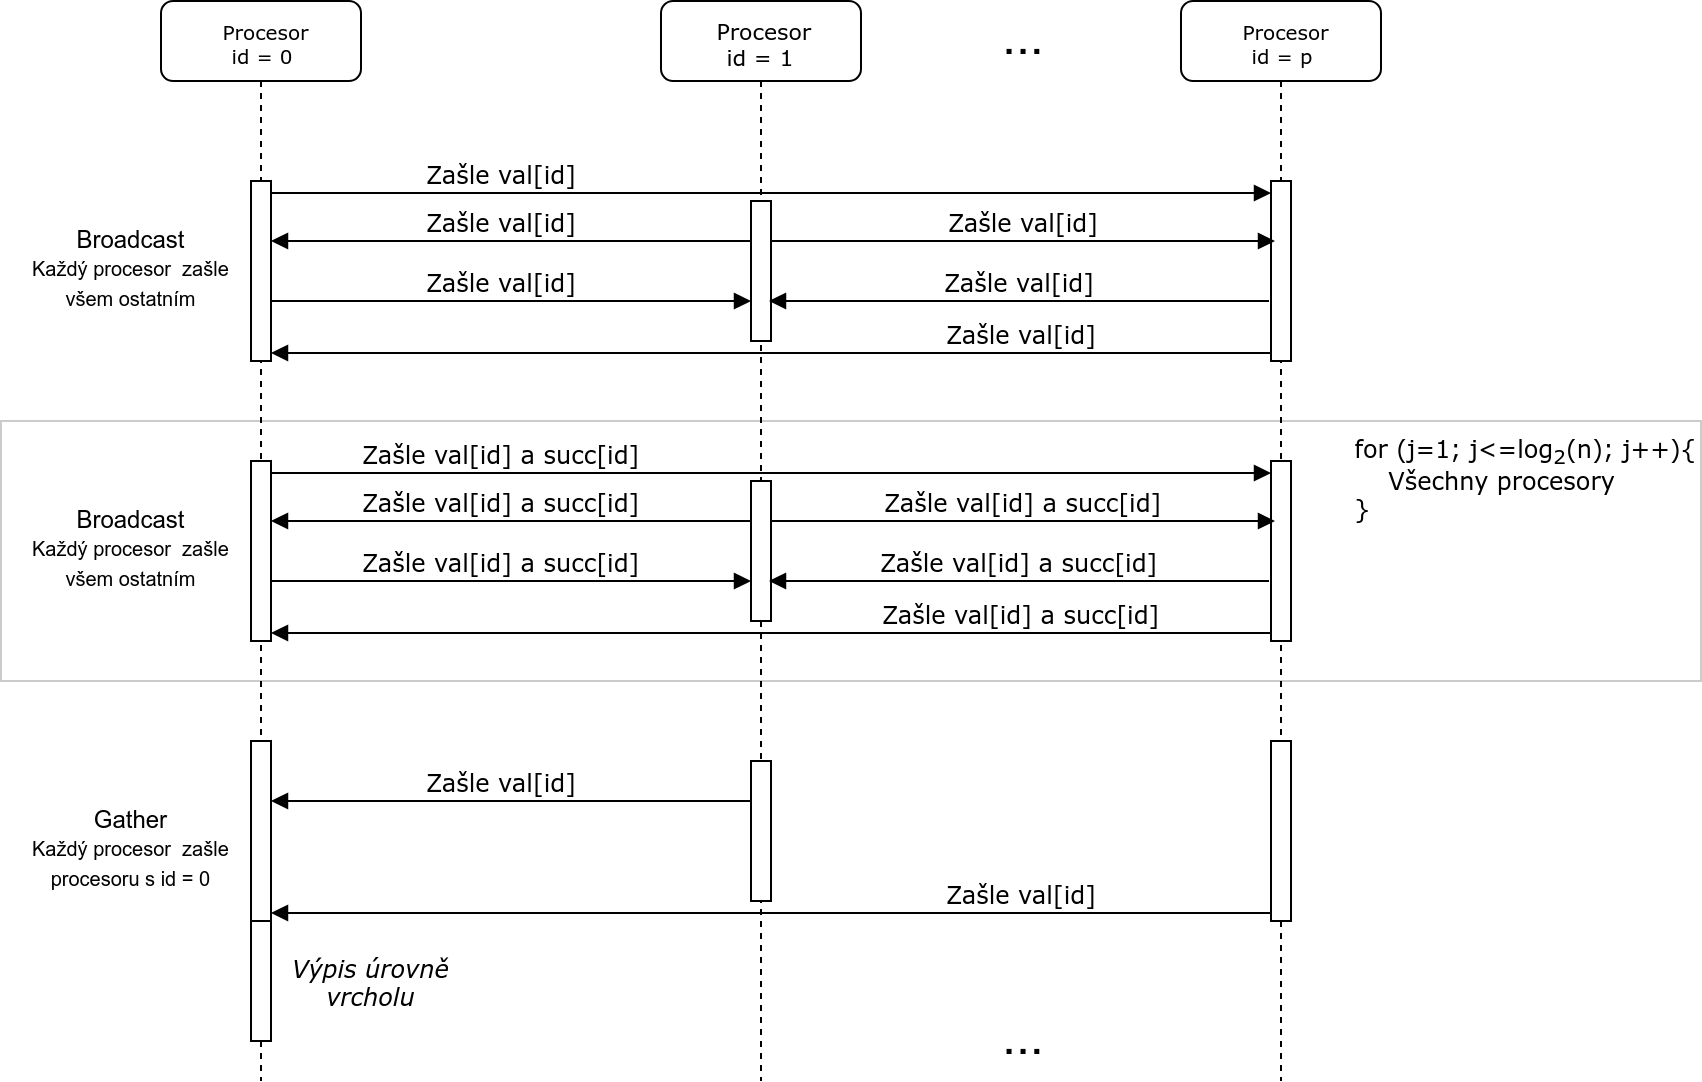
\includegraphics[scale=0.25]{pics/seq.png}
	\caption{Sekvenční diagram komunikace procesorů}	
\end{figure}


\section{Závěr}
V kapitole experimentů z grafu plyne, že algoritmus má sice rychle rostoucí tendenci při aplikaci na malém počtu uzlů, ale při aplikaci na více uzlech se časový průběh postupně mění na logaritmický, což potvrzuje odhad časové složitosti z rozboru a analýzy algoritmu, který byl určen jako $O(log_{2}(n))$. Experimenty byly prováděny na školním serveru Merlin s operačním systémem CentOS.
\end{document}